\begin{figure}
    \centering
    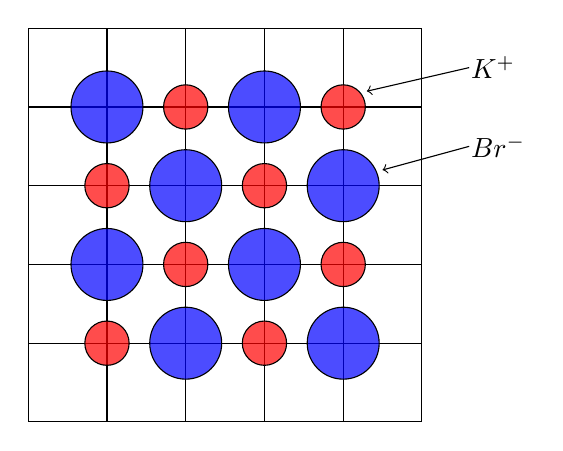
\begin{tikzpicture}
        %grid
        \draw[step=1.0,black,thin] (0,0) grid (5,5);
        %ions
        \filldraw[fill opacity=0.7, fill=red] (1,1) circle (8pt);
        \filldraw[fill opacity=0.7, fill=blue] (2,1) circle (13pt);
        \filldraw[fill opacity=0.7, fill=red] (3,1) circle (8pt);
        \filldraw[fill opacity=0.7, fill=blue] (4,1) circle (13pt);
        \filldraw[fill opacity=0.7, fill=blue] (1,2) circle (13pt);
        \filldraw[fill opacity=0.7, fill=red] (2,2) circle (8pt);
        \filldraw[fill opacity=0.7, fill=blue] (3,2) circle (13pt);
        \filldraw[fill opacity=0.7, fill=red] (4,2) circle (8pt);
        \filldraw[fill opacity=0.7, fill=red] (1,3) circle (8pt);
        \filldraw[fill opacity=0.7, fill=blue] (2,3) circle (13pt);
        \filldraw[fill opacity=0.7, fill=red] (3,3) circle (8pt);
        \filldraw[fill opacity=0.7, fill=blue] (4,3) circle (13pt);
        \filldraw[fill opacity=0.7, fill=blue] (1,4) circle (13pt);
        \filldraw[fill opacity=0.7, fill=red] (2,4) circle (8pt);
        \filldraw[fill opacity=0.7, fill=blue] (3,4) circle (13pt);
        \filldraw[fill opacity=0.7, fill=red] (4,4) circle (8pt);
        %nodes
        \draw (5.5, 4.5) node[right] {$K^{+}$};
        \draw[->] (5.6, 4.5) -- (4.3, 4.2); 
        \draw (5.5, 3.5) node[right] {$Br^{-}$};
        \draw[->] (5.6, 3.5) -- (4.5, 3.2);
    \end{tikzpicture}
    \caption{Form eines KBr Ionenkristalls.}
    \label{fig:probeBild}
\end{figure}
